\chapter{Penggalian Data}
\label{chap:penggalian data}
Pada bab ini akan dijelaskan analisis masalah penelitian ini. Analisis meliputi Langkah-Langkah Query Yang Dilakukan Dengan Data Yang Lebih Besar.

\section{Langkah-Langkah Query Yang Dilakukan Dengan Data Yang Lebih Besar}
Pada section ini akan dijelaskan tentang langkah-langkah query yang dilakukan dalam memperoleh data dan analisis yang dilakukan. Data yang diambil adalah semua data yang akan didapatkan dengan menggunakan \textit{query}. Data yang diambil merupakan dataset dari tabel technologies 2020$\_$08$\_$01:

\subsection{Mengumpulkan List Website}
Langkah pertama yang dilakukan yaitu mengumpulkan website. Website yang dicari tidak berdasarkan berdasarkan \textit{rank} karena tidak tersedia pada dataset tersebut. Berikut adalah \textit{query} yang digunakan untuk mengumpulkan list website.
\begin{verbatim}
	SELECT url
	FROM `httparchive.technologies.2020_08_01_*`
	ORDER BY url asc
\end{verbatim}

\subsection{Mencari Aplikasi Yang Digunakan Website}
Setiap website akan dicari aplikasi apa saja yang digunakan dalam pembangunan website tersebut dan versi dari aplikasi yang dipakainya. Berikut adalah query yang digunakan.
\begin{verbatim}
	SELECT url, app, info
	FROM `httparchive.technologies.2020_08_01_*`
	ORDER BY url asc
\end{verbatim}

\subsection{Mengelompokkan Berdasarkan Nama Semua Aplikasi Yang Dipakai}
Pengelompokan aplikasi dapat dilakukan dengan menggunakan query. Berikut adalah query yang digunakan.
\begin{verbatim}
	SELECT tabelName.app, num.num_sites , versioned.versioned_count , unversioned.unversioned_count
	FROM 
	(SELECT DISTINCT app
	FROM `httparchive.technologies.2020_08_01_*` ) tabelName
	
	LEFT JOIN 
	
	(SELECT tabel1.app, count(app) AS versioned_count
	FROM `httparchive.technologies.2020_08_01_*` AS tabel1
	WHERE tabel1.app!="" AND tabel1.info != "" 
	GROUP BY tabel1.app) AS versioned
	
	ON(versioned.app = tabelName.app)
	
	LEFT JOIN
	
	(SELECT tabel2.app, count(app) AS unversioned_count
	FROM `httparchive.technologies.2020_08_01_*` AS tabel2
	WHERE tabel2.app!="" AND tabel2.info = "" 
	GROUP BY tabel2.app) AS unversioned
	
	ON (unversioned.app = tabelName.app)
	
	LEFT JOIN 
	
	(SELECT app, count(url) AS num_sites
	FROM `httparchive.technologies.2020_08_01_*`
	GROUP BY app) AS num
	
	ON (tabelName.app = num.app)
\end{verbatim}

\subsection{Mencari Data Tentang Versi Aplikasi Yang Masih Didukung}
Sebelum menentukan suatau aplikasi usang atau tidak, kita harus mencari versi dari setiap aplikasi secara manual. Versi setiap aplikasi dapat dilihat di-\textit{official documentation} dari setiap aplikasi. Hasil pencarian dari aplikasi yang masih didukung dapat dilihat pada gambar \ref{appData}. 

\subsection{Melakukan Perbandingan Antara Versi Aplikasi Yang Masih Dipakai Sekarang Dengan Versi Aplikasi Yang Masih Didukung}


\section{Hasil Sample Data}
Data yang ditampilkan adalah data beberapa aplikasi yang sudah dipisahkan berdasarkan aplikasi dan nomor versi dari aplikasi yang dipakai serta jumlahnya dalam bentuk \textit{chart}.
\subsection{Cherokee}
Berikut ini adalah chart yang dapat dilihat:
\begin{figure}[H]
	\centering  
	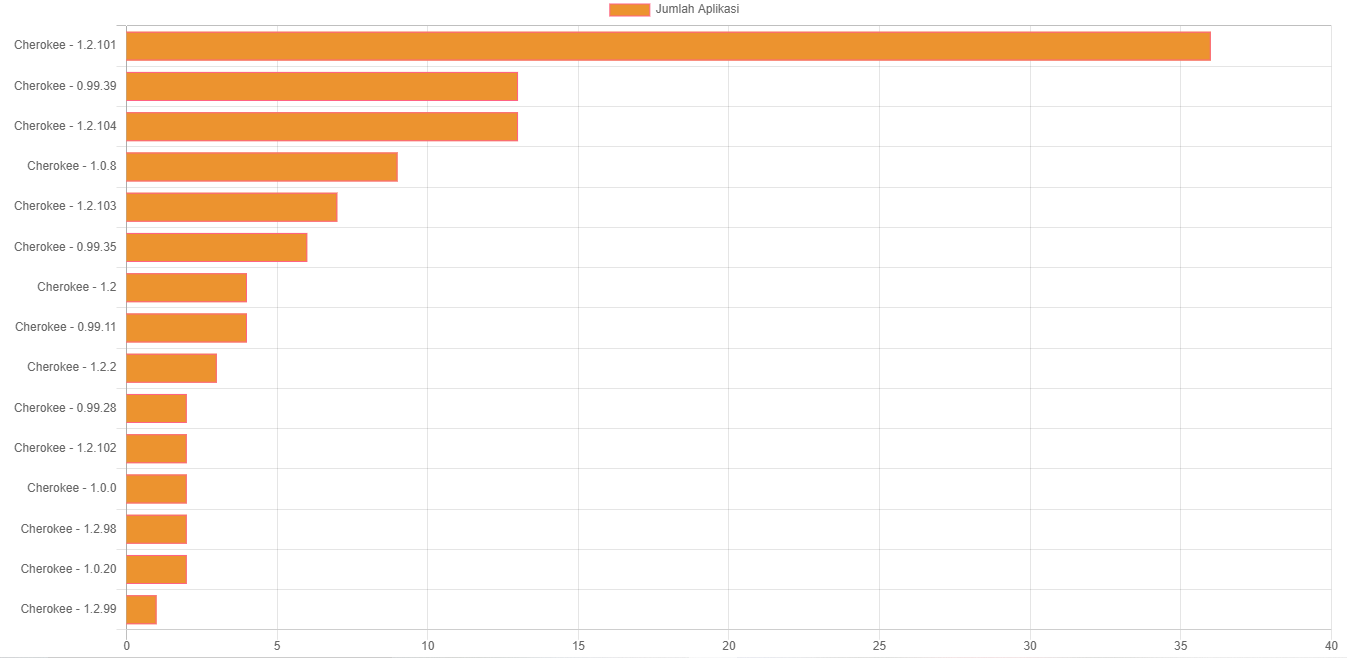
\includegraphics[scale=0.5]{Gambar/hasil_chart_cherokee.PNG}  
	\caption{Aplikasi Cherokee} 
	\label{fig:data_sample_cherokee} 
\end{figure}
\subsection{Angular Material}
Berikut ini adalah chart yang dapat dilihat:
\begin{figure}[H]
	\centering  
	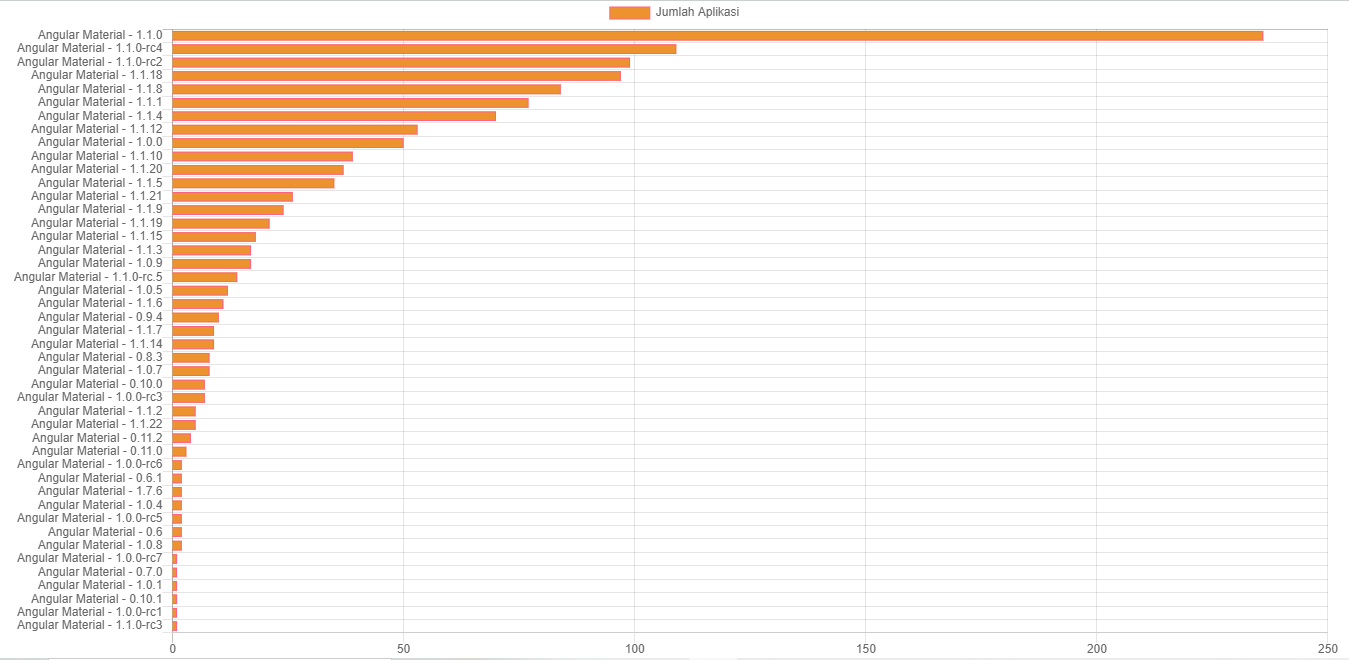
\includegraphics[scale=0.5]{Gambar/hasil_chart_angular.PNG}  
	\caption{Aplikasi Angular Material} 
	\label{fig:data_sample_angular} 
\end{figure}
